\documentclass{article}
\usepackage{graphicx}
\usepackage{siunitx}
\graphicspath{ {images/} }
\title{Football Forces}
\author{Grant Curell}
\begin{document}
\maketitle{}
\section{Problem}
Slipping intrepidly into the mass of moving players, risking injury in the name of science, you measure the magnitude of these forces and mark them down on your clipboard: Fa = 15.0 N Fb = 12.5 N Fc = 16.5 N You measure the mass of the football as 0.40 kilograms (I don’t include the force of gravity). Now you wonder where the football will be in 1.0 second, assuming the forces shown act on the ball continuously during that second.

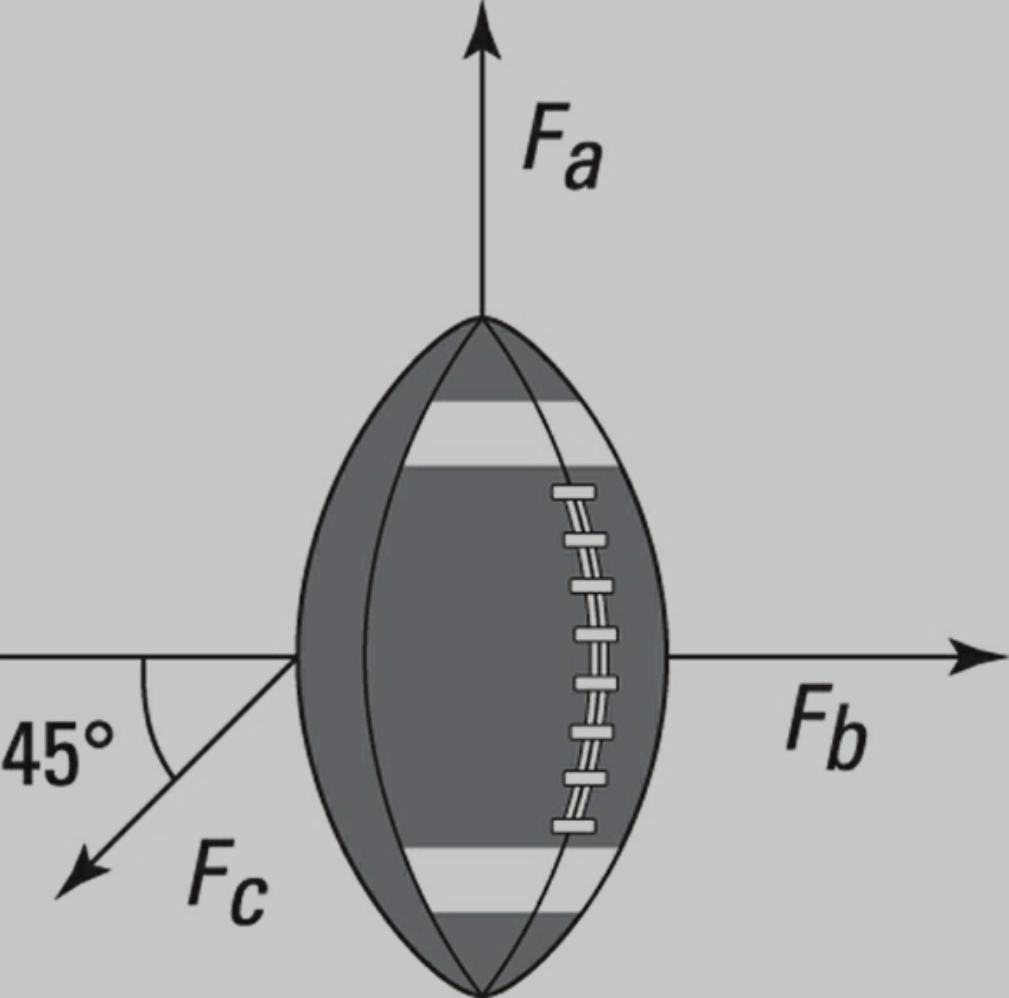
\includegraphics[width=\columnwidth]{image}
\\\\
Holzner, Steven. Physics I For Dummies (For Dummies (Math \& Science)) (p. 86). Wiley. Kindle Edition.
\\\\
\section{Solution}
\[ F_a = 15.0N \]
\[ F_b = 12.5N \]
\[ F_c = 16.5N \]
\[ 15\cos(90)+12.5\cos(0)+16.5\cos(225)=.832 \]
\[ 15\sin(90)+12.5\sin(0)+16.5\sin(225)=3.332 \]
\[ \sum F=ma \]
\[ \frac{.832}{.4}=a \]
\[ a=\frac{\triangle{v}}{\triangle{t}} \]
\[ v_{fx}=\frac{.832}{.4}*1 \]
\[ \bar{v_x} = \frac{v_{ix}+v_{fx}}{2} \]
\[ \bar{v_x} = \frac{0+\frac{.832}{.4}*1}{2} \]
\[ \bar{v_x} = 1m/s \]
\[ s_x=\bar{v_x}t \]
\[ s_x=1*1 \]
\[ s_x=1m \]
Repetiendo exactamente el mismo processo para y
\[ s_y=4.2m \]

\end{document}
